\subsection{Versuchsaufbau}
%skizze zum versuchsaufbau (oder foto) einf�gen,   es muss erkl�rt werden wie das ganze funktioniert und welche speziellen einstellungen verwendet wurden (z.b. welche kn�pfe an den ger�ten f�r die messung verdreht wurden)

\begin{figure}[H]
\centering
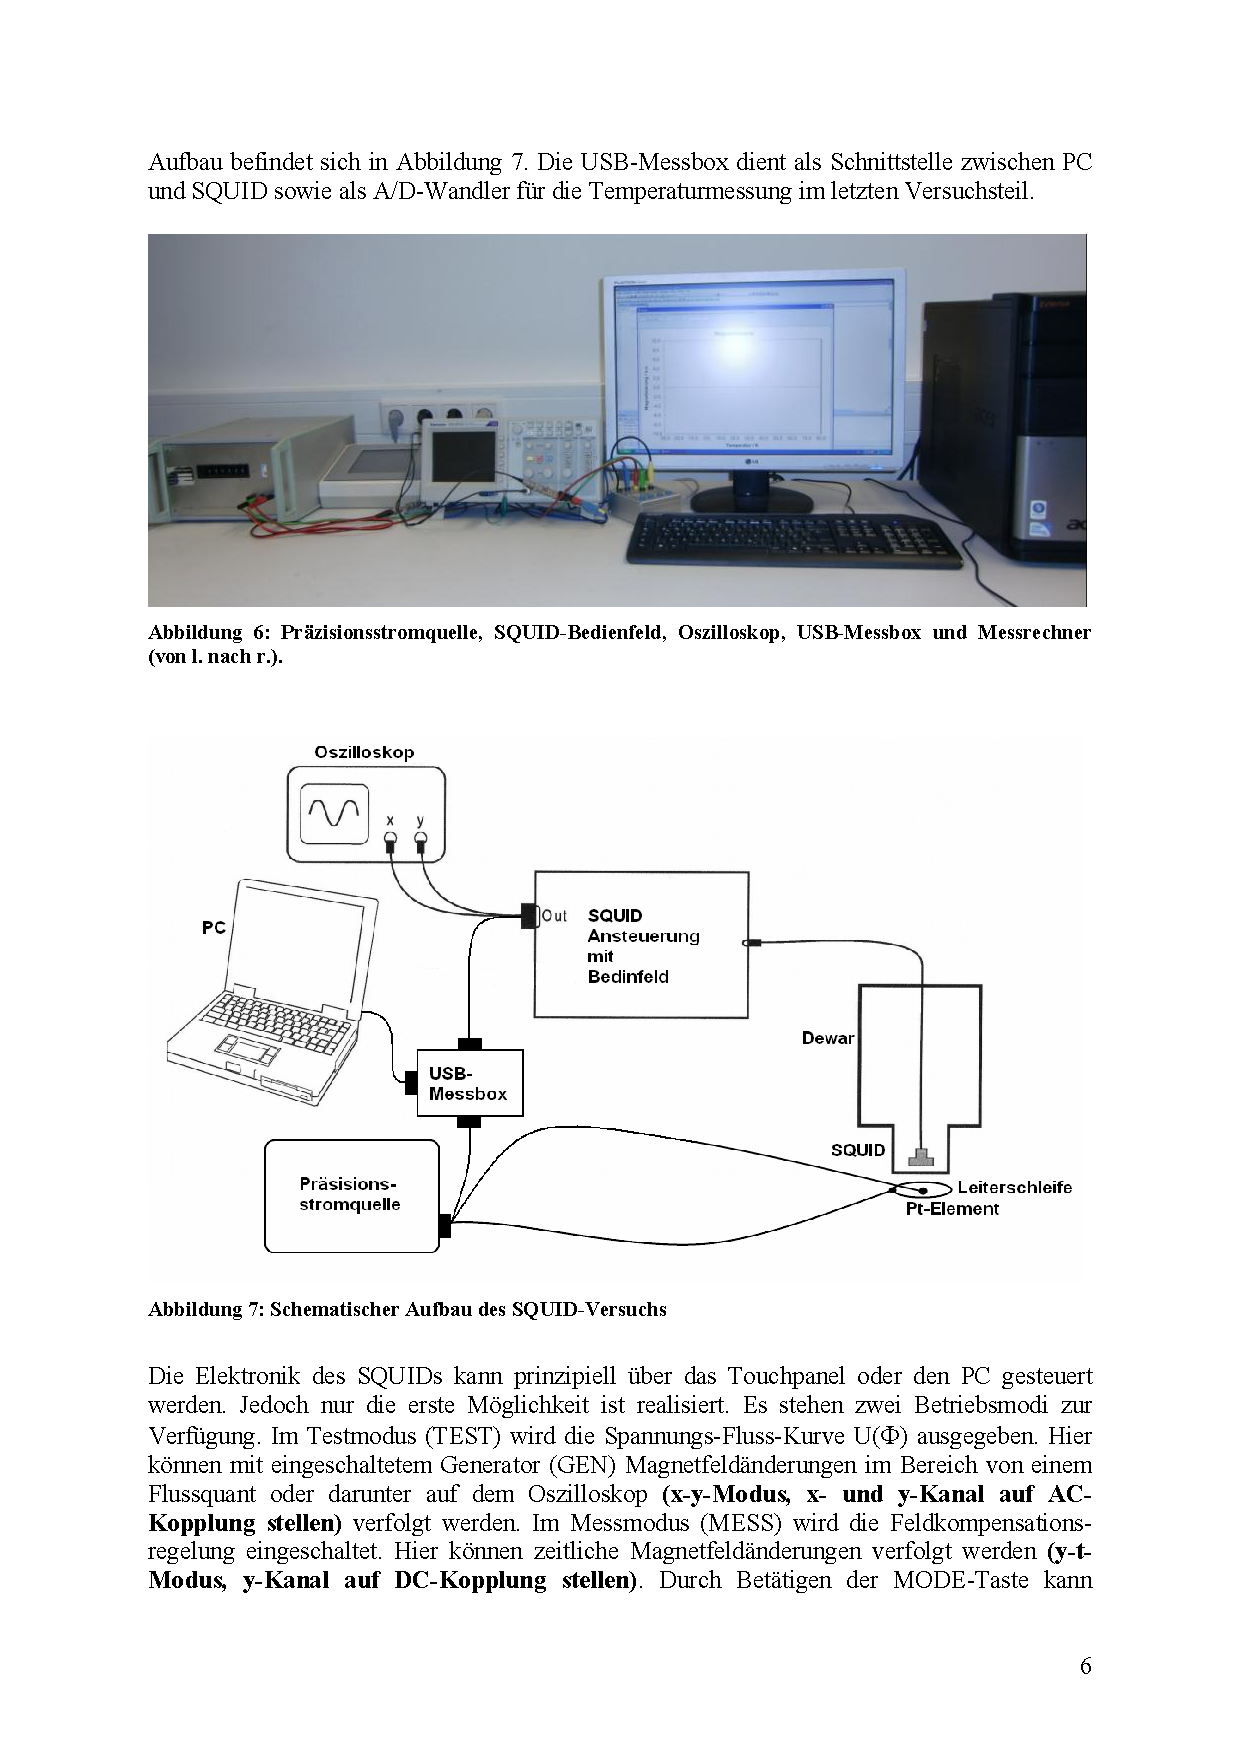
\includegraphics[scale = 1,trim = 10mm 80mm 10mm 120mm, clip]{aufbau_1}
\caption{Aufbau des Experiments \cite{Schematischer_Aufbau}}
\label{fig:schem_auf}
\end{figure}